%
% CSE Electronic Homework Template
% Last modified 8/23/2018 by Jeremy Buhler

\documentclass[11pt]{article}
\usepackage[left=0.7in,right=0.7in,top=1in,bottom=0.7in]{geometry}
\usepackage{fancyhdr} % for header
\usepackage{graphicx} % for figures
\usepackage{amsmath}  % for extended math markup
\usepackage{amssymb}
\usepackage[bookmarks=false]{hyperref} % for URL embedding
\usepackage[noend]{algpseudocode} % for pseudocode
\usepackage[plain]{algorithm} % float environment for algorithms

%%%%%%%%%%%%%%%%%%%%%%%%%%%%%%%%%%%%%%%%%%%%%%%%%%%%%%%%%%%%%%%%%%%%%%
% STUDENT: modify the following fields to reflect your
% name/ID, the current homework, and the current problem number

% Example: 
%\newcommand{\StudentName}{Jeremy Buhler}
%\newcommand{\StudentID{123456}

\newcommand{\StudentName}{Dingyu Wang (Howard)}
\newcommand{\StudentID}{COMP 642: Machine Learning}
\newcommand{\HomeworkNumber}{8}

%%%%%%%%%%%%%%%%%%%%%%%%%%%%%%%%%%%%%%%%%%%%%%%%%%%%%%%%%%%%%%%%%%%%%%%%
% You can pretty much leave the stuff up to the next line of %%'s alone.

% create header and footer for every page
\pagestyle{fancy}
\fancyhf{}
\lhead{\textbf{\StudentName}}
\chead{\textbf{\StudentID}}
\rhead{\textbf{HW \HomeworkNumber}}
\cfoot{\thepage}

% preferred pseudocode style
\algrenewcommand{\algorithmicprocedure}{}
\algrenewcommand{\algorithmicthen}{}

% ``do { ... } while (cond)''
\algdef{SE}[DOWHILE]{Do}{doWhile}{\algorithmicdo}[1]{\algorithmicwhile\ #1}%

% ``for (x in y ... z)''
\newcommand{\ForRange}[3]{\For{#1 \textbf{in} #2 \ \ldots \ #3}}

% these are common math formatting commands that aren't defined by default
\newcommand{\union}{\cup}
\newcommand{\isect}{\cap}
\newcommand{\ceil}[1]{\ensuremath \left\lceil #1 \right\rceil}
\newcommand{\floor}[1]{\ensuremath \left\lfloor #1 \right\rfloor}

%%%%%%%%%%%%%%%%%%%%%%%%%%%%%%%%%%%%%%%%%%%%%%%%%%%%%%%%%%%%%%%%%%%%%%
\usepackage[utf8]{inputenc}
\usepackage[english]{babel}
\setlength{\parindent}{0em}
\setlength{\parskip}{1em}
 \usepackage{pythonhighlight}
\usepackage{graphicx}
\graphicspath{ {./images/} }


\begin{document}
1) \\
between input layer and hidden layer 1 = 4 x 5 = 20 \\
between hidden layer 1 and hidden layer 2 = 5 x 3 = 15 \\
between hidden layer 2 and output = 3 x 1 = 3 \\
20 + 15 + 3 = 38 \\
38 trainable parameters.

2) \\
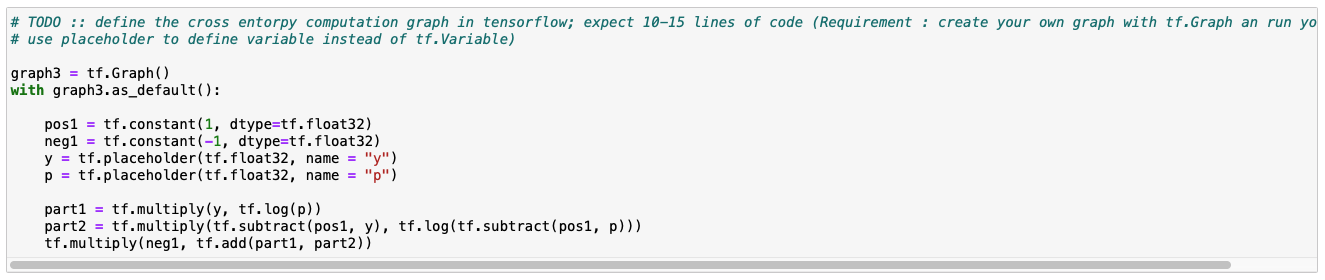
\includegraphics[scale= 0.35]{tf1new} \\
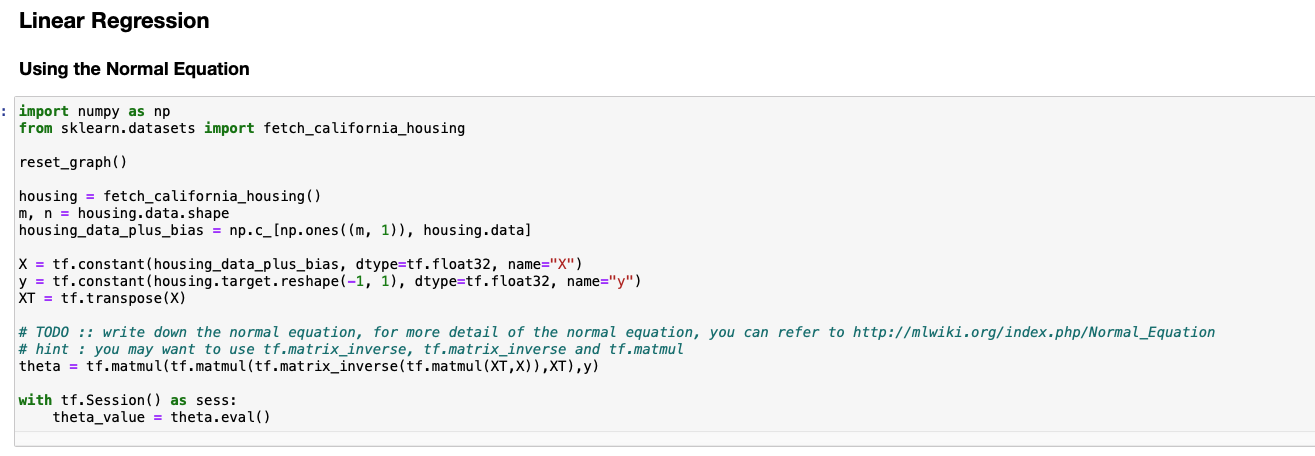
\includegraphics[scale= 0.35]{tf2} \\
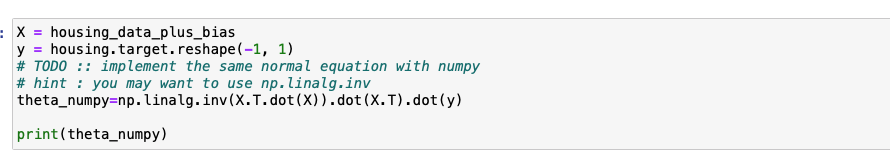
\includegraphics[scale= 0.35]{tf3} \\
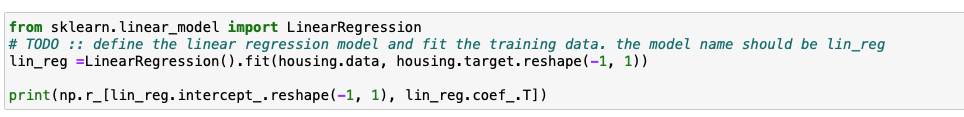
\includegraphics[scale= 0.35]{tf4} \\
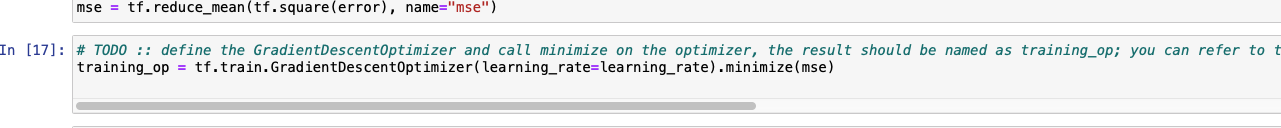
\includegraphics[scale= 0.35]{tf5} \\
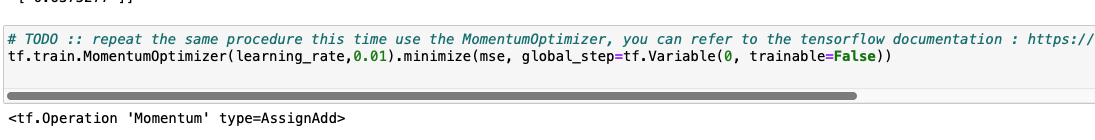
\includegraphics[scale= 0.35]{tf6} \\
\\ \\ \\ \\ \\ \\


3) \\
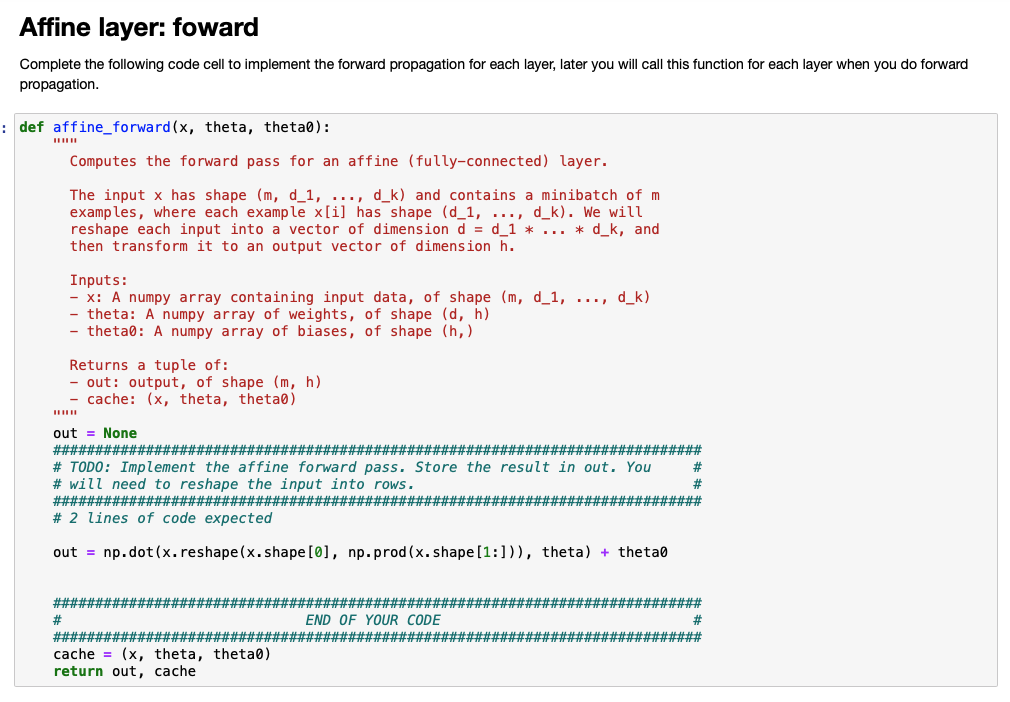
\includegraphics[scale= 0.35]{hw8-1} \\
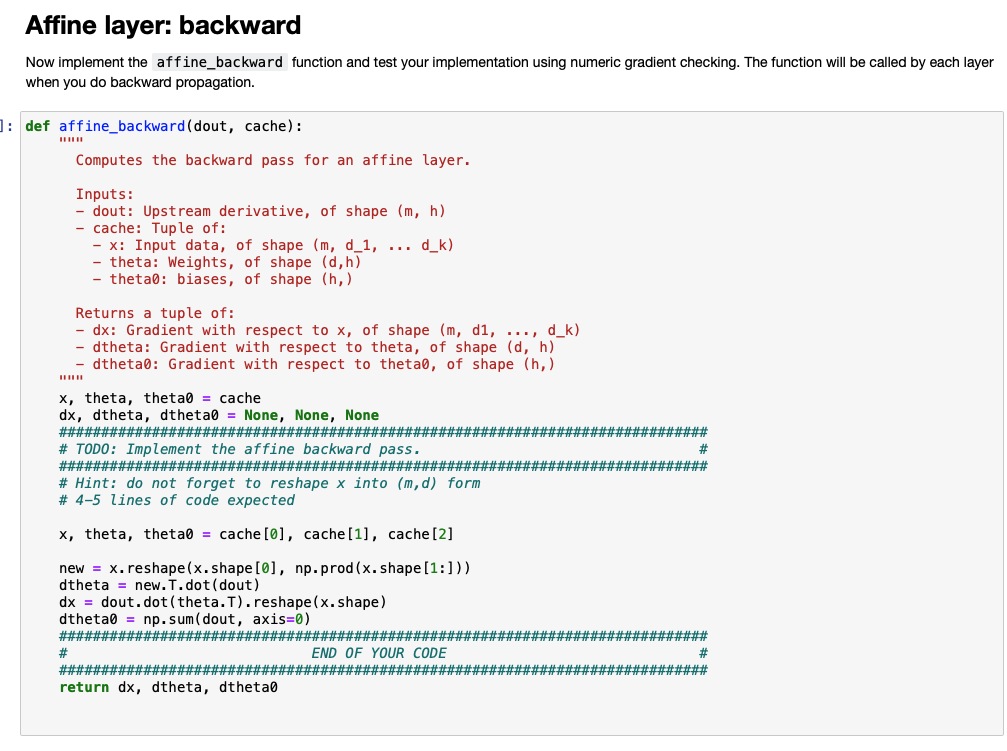
\includegraphics[scale= 0.35]{hw8-2} \\
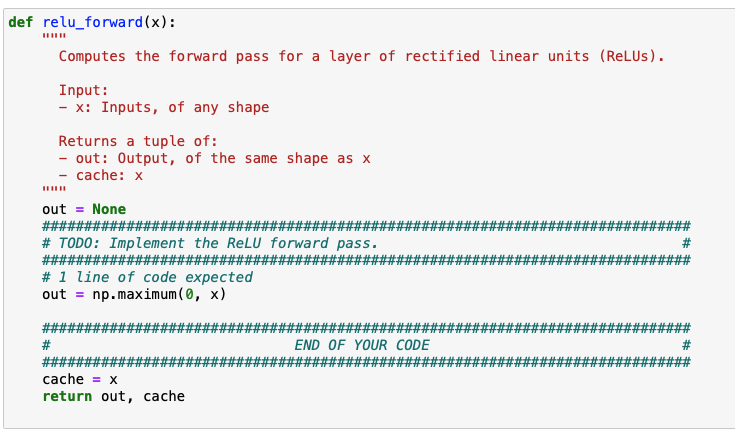
\includegraphics[scale= 0.35]{hw8-3} \\
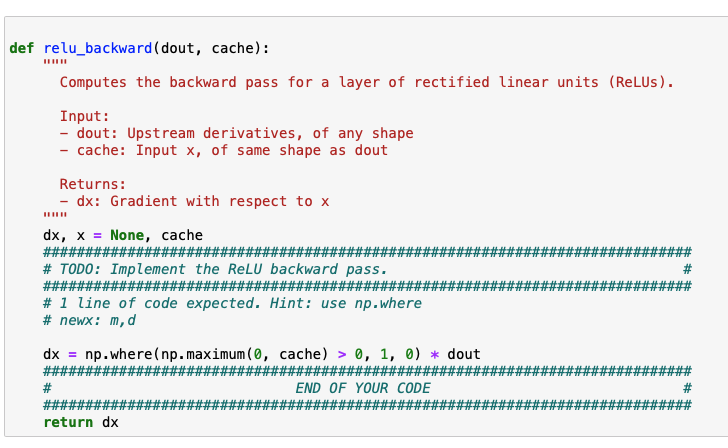
\includegraphics[scale= 0.35]{hw8-4} \\
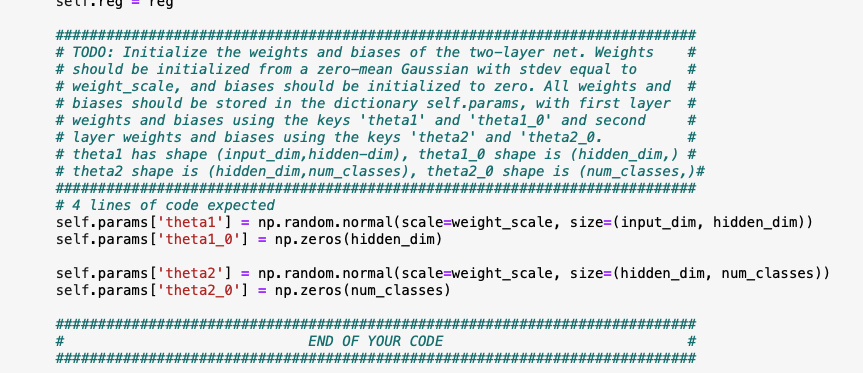
\includegraphics[scale= 0.35]{hw8-5} \\
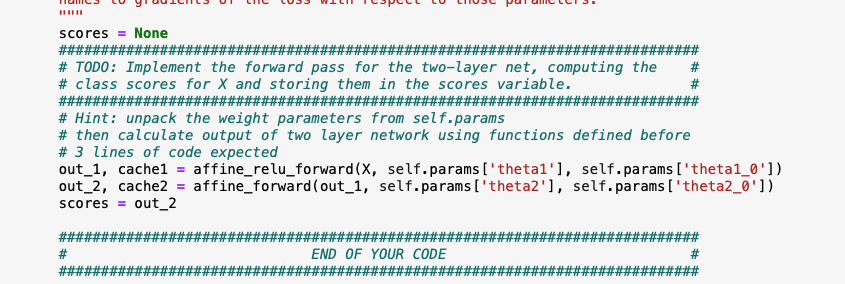
\includegraphics[scale= 0.35]{hw8-6} \\
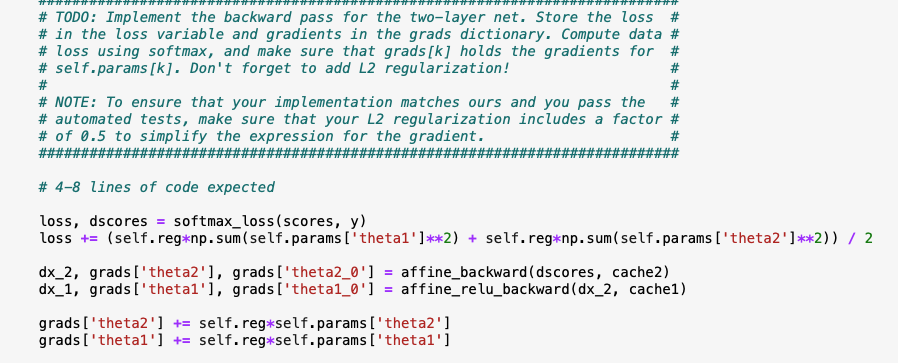
\includegraphics[scale= 0.35]{hw8-7} \\
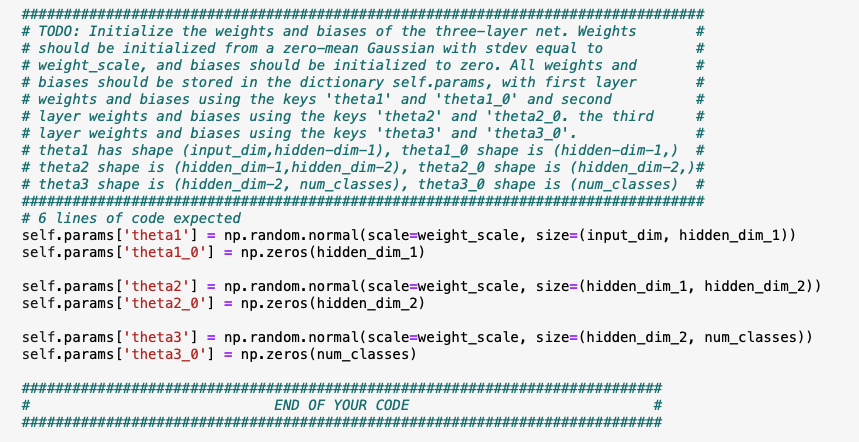
\includegraphics[scale= 0.35]{hw8-8} \\
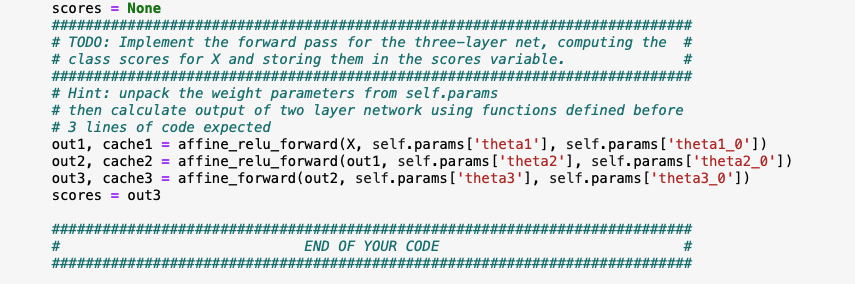
\includegraphics[scale= 0.35]{hw8-9} \\
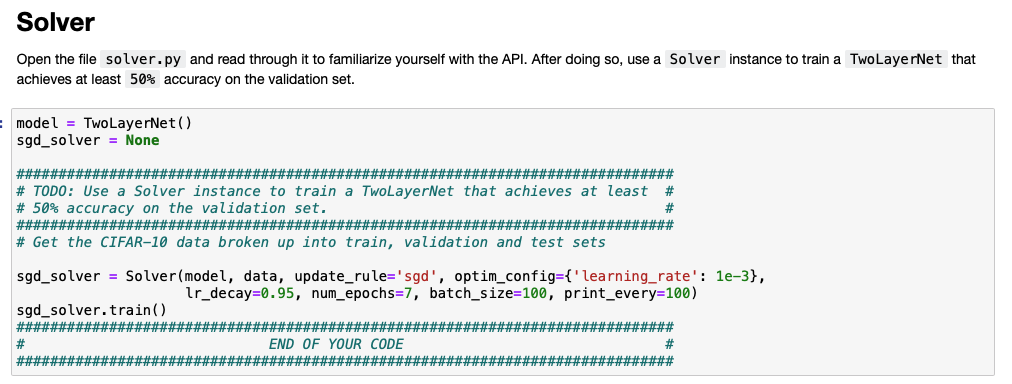
\includegraphics[scale= 0.35]{hw8-10} \\
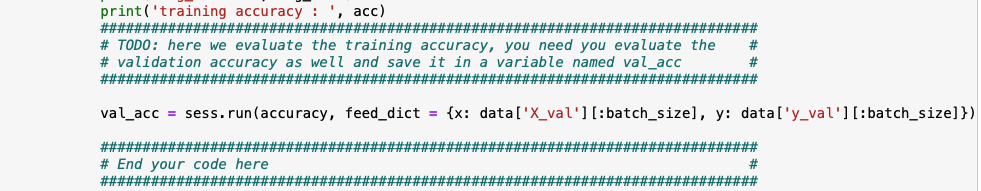
\includegraphics[scale= 0.35]{hw8-11} \\
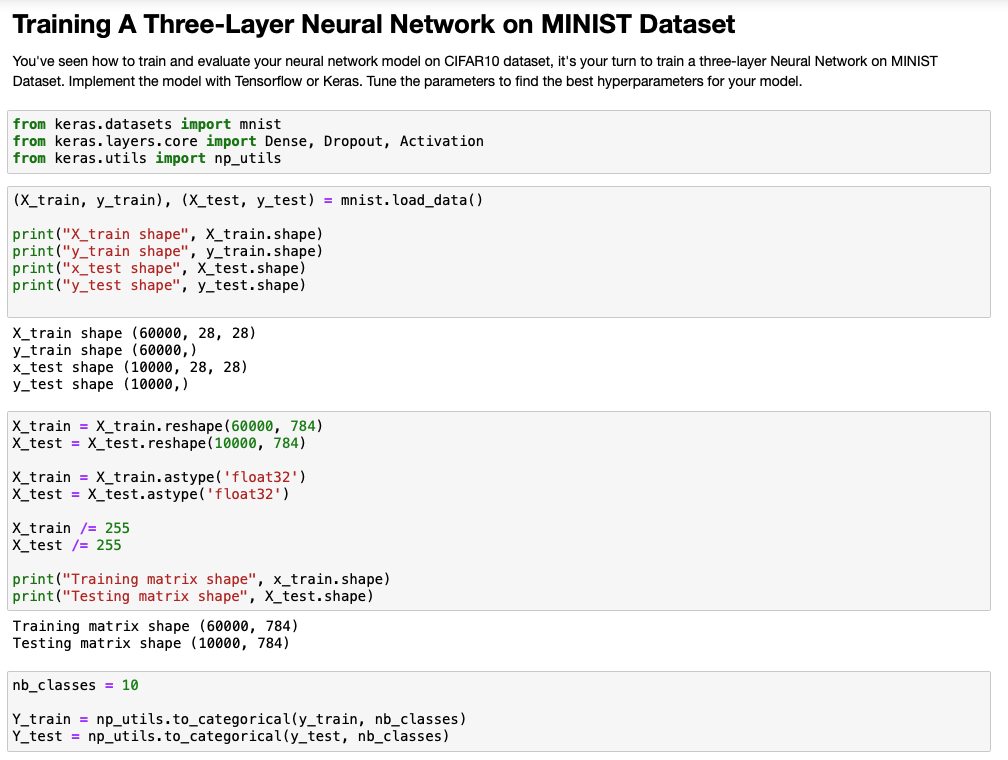
\includegraphics[scale= 0.35]{hw8-20} \\
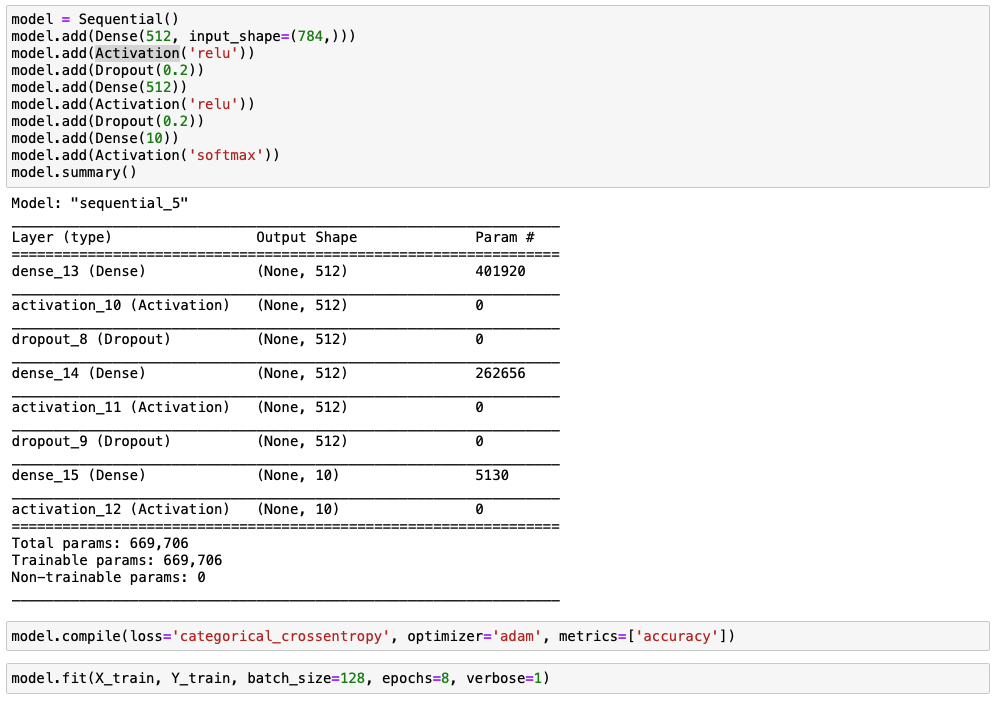
\includegraphics[scale= 0.35]{hw8-21} \\
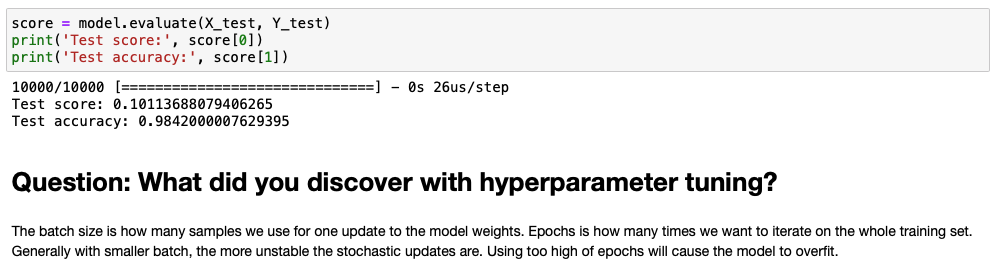
\includegraphics[scale= 0.35]{hw8-22} \\
\end{document}

